\subsection{\textsc{Mnist}}
\begin{figure}[H]
    \centering
    \begin{subfigure}{.32\textwidth}
        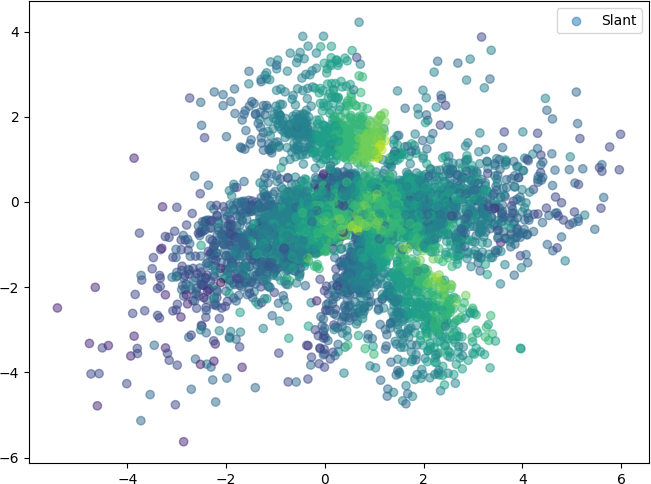
\includegraphics[width=\textwidth]{images/latent_spaces/mnist/vae_gan/embeddings_mu_0.png}
        \caption{Latent space colored by digit slant}
    \end{subfigure}
    \hfill
    \begin{subfigure}{.32\textwidth}
        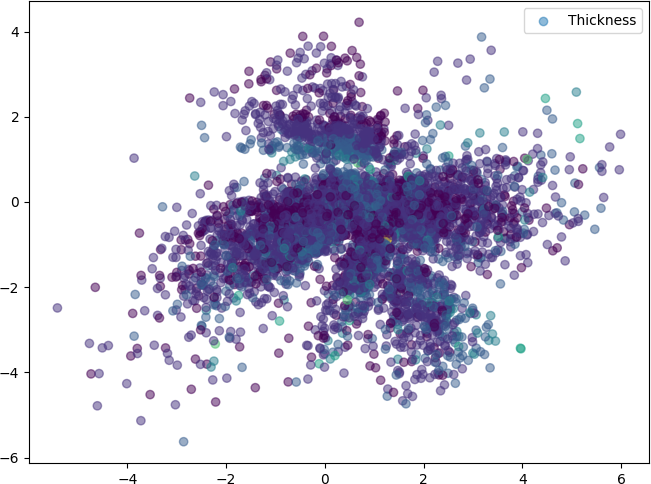
\includegraphics[width=\textwidth]{images/latent_spaces/mnist/vae_gan/embeddings_mu_1.png}
        \caption{Latent space colored by digit thickness}
    \end{subfigure}
    \hfill
    \begin{subfigure}{.32\textwidth}
        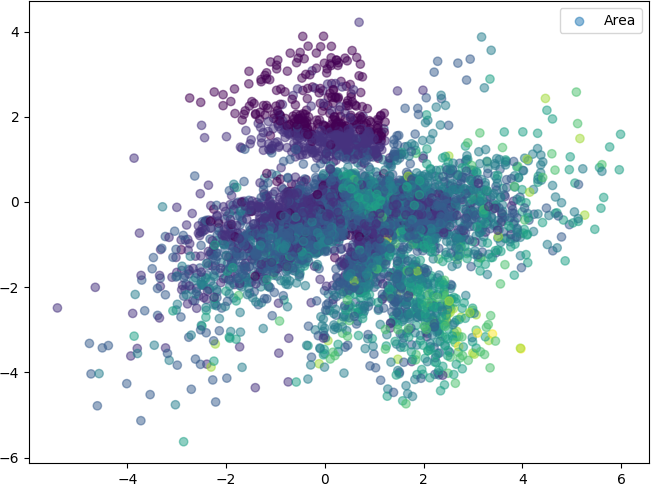
\includegraphics[width=\textwidth]{images/latent_spaces/mnist/vae_gan/embeddings_mu_2.png}
        \caption{Latent space colored by digit area}
    \end{subfigure}
    \hfill
    \begin{subfigure}{.24\textwidth}
        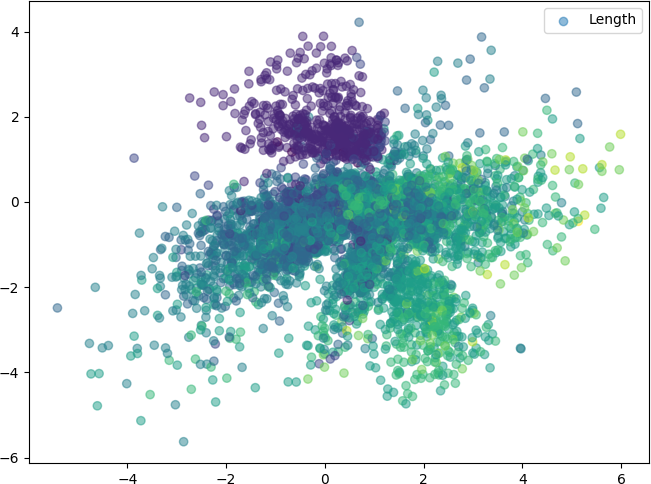
\includegraphics[width=\textwidth]{images/latent_spaces/mnist/vae_gan/embeddings_mu_3.png}
        \caption{Latent space colored by digit length}
    \end{subfigure}
    \hfill
    \begin{subfigure}{.24\textwidth}
        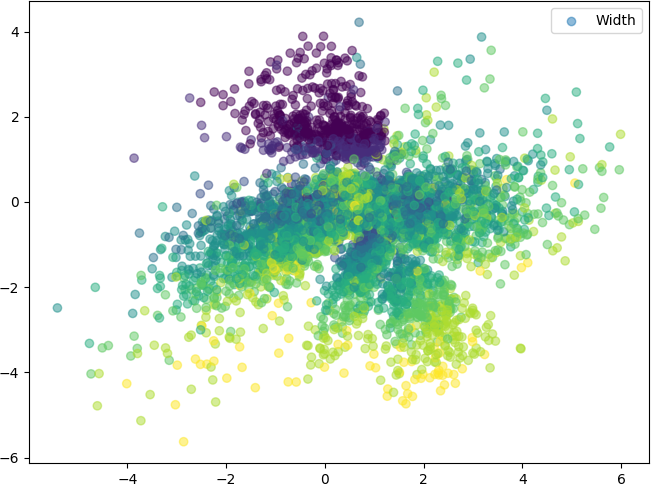
\includegraphics[width=\textwidth]{images/latent_spaces/mnist/vae_gan/embeddings_mu_4.png}
        \caption{Latent space colored by digit width}
    \end{subfigure}
    \hfill
    \begin{subfigure}{.24\textwidth}
        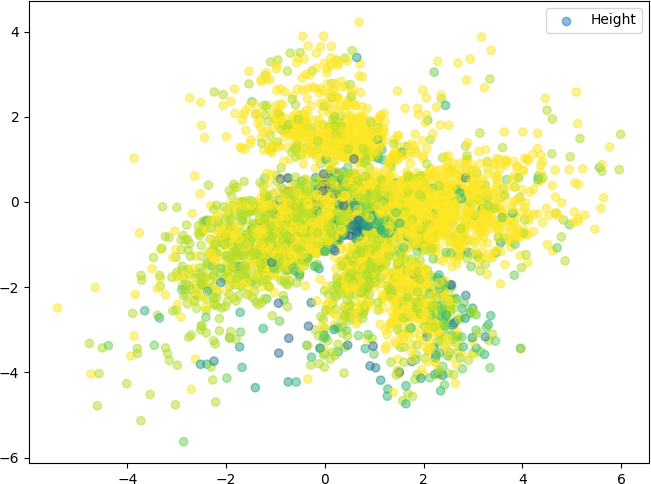
\includegraphics[width=\textwidth]{images/latent_spaces/mnist/vae_gan/embeddings_mu_5.png}
        \caption{Latent space colored by digit height}
    \end{subfigure}
    \hfill
    \begin{subfigure}{.24\textwidth}
        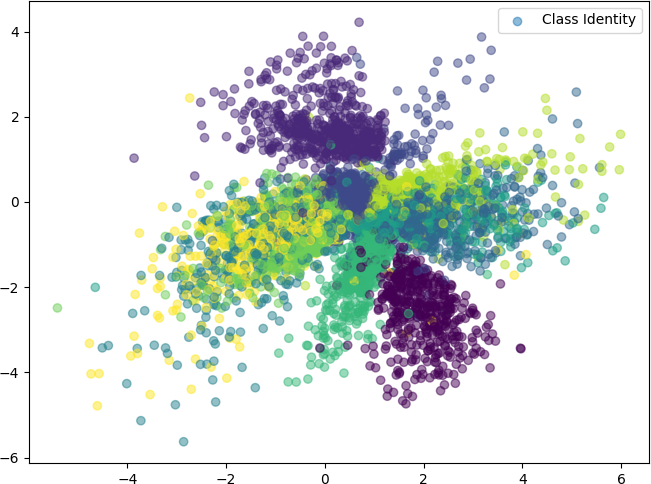
\includegraphics[width=\textwidth]{images/latent_spaces/mnist/vae_gan/embeddings_mu_6.png}
        \caption{Latent space colored by digit identity}
    \end{subfigure}
    \caption[\textsc{Mnist}-VAE-GAN - Latent Space]{Latent space colored by different means of \textsc{Mnist}-\ac{VAE}-\ac{GAN}}
    \label{fig:vae_gan_latent_space_mnist}
\end{figure}

\begin{landscape}
    \begin{figure}[H]
        \centering
        \foreach \i in {1,2,3}{
        \begin{adjustbox}{valign=T}
            \begin{subfigure}{.19\textwidth}
                \includegraphics[width=\textwidth]{images/latent_spaces/mnist/vlae_gan/embeddings_mu_\i_0.png}
                \caption{$z_{\i}$: digit slant}
            \end{subfigure}
        \end{adjustbox}
        \hfill
        \begin{adjustbox}{valign=T}
            \begin{subfigure}{.19\textwidth}
                \includegraphics[width=\textwidth]{images/latent_spaces/mnist/vlae_gan/embeddings_mu_\i_1.png}
                \caption{$z_{\i}$: digit thickness}
            \end{subfigure}
        \end{adjustbox}
        \hfill
        \begin{adjustbox}{valign=T}
            \begin{subfigure}{.19\textwidth}
                \includegraphics[width=\textwidth]{images/latent_spaces/mnist/vlae_gan/embeddings_mu_\i_2.png}
                \caption{$z_{\i}$: digit area}
            \end{subfigure}
        \end{adjustbox}
        \hfill
        \begin{adjustbox}{valign=T}
            \begin{subfigure}{.19\textwidth}
                \includegraphics[width=\textwidth]{images/latent_spaces/mnist/vlae_gan/embeddings_mu_\i_3.png}
                \caption{$z_{\i}$: digit length}
            \end{subfigure}
        \end{adjustbox}
        \hfill
        \begin{adjustbox}{valign=T}
            \begin{subfigure}{.19\textwidth}
                \includegraphics[width=\textwidth]{images/latent_spaces/mnist/vlae_gan/embeddings_mu_\i_4.png}
                \caption{$z_{\i}$: digit width}
            \end{subfigure}
        \end{adjustbox}
        \hfill
        \begin{adjustbox}{valign=T}
            \begin{subfigure}{.19\textwidth}
                \includegraphics[width=\textwidth]{images/latent_spaces/mnist/vlae_gan/embeddings_mu_\i_5.png}
                \caption{$z_{\i}$: digit height}
            \end{subfigure}
        \end{adjustbox}
        \hfill
        \begin{adjustbox}{valign=T}
            \begin{subfigure}{.19\textwidth}
                \includegraphics[width=\textwidth]{images/latent_spaces/mnist/vlae_gan/embeddings_mu_\i_6.png}
                \caption{$z_{\i}$: digit identity}
            \end{subfigure}
        \end{adjustbox}}
        \caption[\textsc{Mnist}-VLAE-GAN - Latent Space]{Latent space colored by different means of \textsc{Mnist}-\ac{VLAE}-\ac{GAN}}
        \label{fig:vlae_gan_latent_space_mnist}
    \end{figure}
\end{landscape}

\subsection{dSprites}
\begin{figure}[H]
    \centering
    \begin{subfigure}{.19\textwidth}
        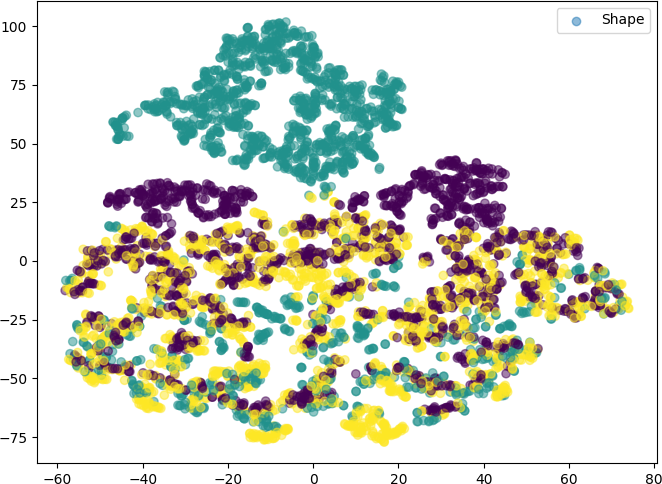
\includegraphics[width=\textwidth]{images/latent_spaces/dsprites/vae_gan/embeddings_mu_0.png}
        \caption{Latent space colored by object shape}
    \end{subfigure}
    \hfill
    \begin{subfigure}{.19\textwidth}
        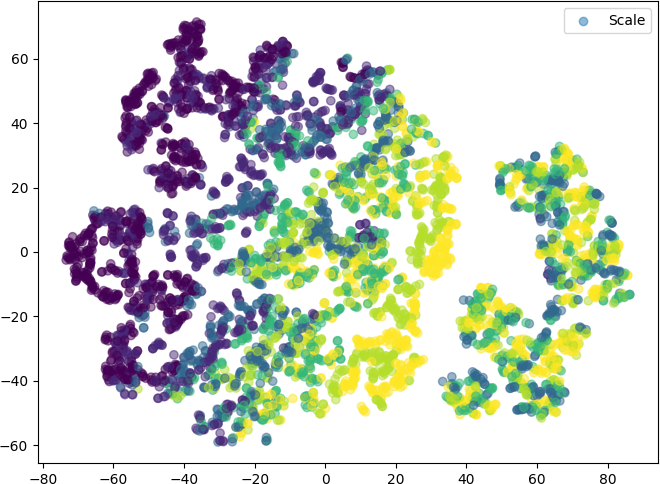
\includegraphics[width=\textwidth]{images/latent_spaces/dsprites/vae_gan/embeddings_mu_1.png}
        \caption{Latent space colored by object scale}
    \end{subfigure}
    \hfill
    \begin{subfigure}{.19\textwidth}
        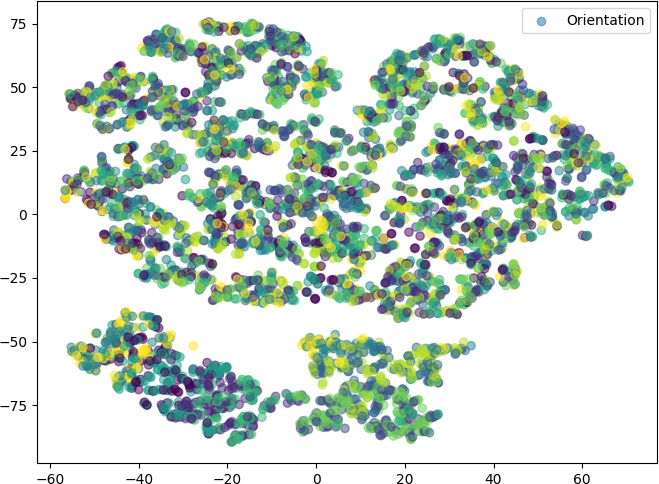
\includegraphics[width=\textwidth]{images/latent_spaces/dsprites/vae_gan/embeddings_mu_2.png}
        \caption{Latent space colored by object orientation}
    \end{subfigure}
    \hfill
    \begin{subfigure}{.19\textwidth}
        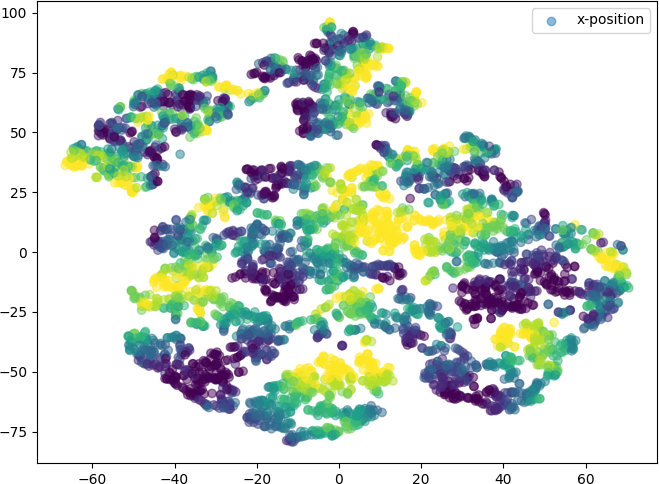
\includegraphics[width=\textwidth]{images/latent_spaces/dsprites/vae_gan/embeddings_mu_3.png}
        \caption{Latent space colored by object $x$-position}
    \end{subfigure}
    \hfill
    \begin{subfigure}{.19\textwidth}
        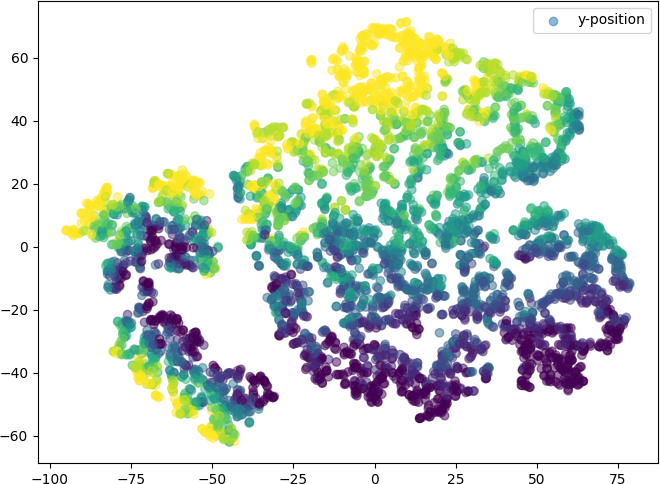
\includegraphics[width=\textwidth]{images/latent_spaces/dsprites/vae_gan/embeddings_mu_4.png}
        \caption{Latent space colored by object $y$-position}
    \end{subfigure}
    \caption[dSprites-VAE-GAN - Latent Space]{\ac{t-SNE}-reduced latent space embeddings colored by different means of dSprites-\ac{VAE}-\ac{GAN}}
    \label{fig:vae_gan_latent_space_dsprites}
\end{figure}
\begin{figure}[H]
    \centering
    \foreach \i in {1,2,3}{
    \begin{subfigure}{.19\textwidth}
        \includegraphics[width=\textwidth]{images/latent_spaces/dsprites/vlae_gan/embeddings_mu_\i_0.png}
        \caption{Latent space $z_{\i}$ colored by object shape}
    \end{subfigure}
    \hfill
    \begin{subfigure}{.19\textwidth}
        \includegraphics[width=\textwidth]{images/latent_spaces/dsprites/vlae_gan/embeddings_mu_\i_1.png}
        \caption{Latent space $z_{\i}$ colored by object scale}
    \end{subfigure}
    \hfill
    \begin{subfigure}{.19\textwidth}
        \includegraphics[width=\textwidth]{images/latent_spaces/dsprites/vlae_gan/embeddings_mu_\i_2.png}
        \caption{Latent space $z_{\i}$ colored by object orientation}
    \end{subfigure}
    \hfill
    \begin{subfigure}{.19\textwidth}
        \includegraphics[width=\textwidth]{images/latent_spaces/dsprites/vlae_gan/embeddings_mu_\i_3.png}
        \caption{Latent space $z_{\i}$ colored by object $x$-position}
    \end{subfigure}
    \hfill
    \begin{subfigure}{.19\textwidth}
        \includegraphics[width=\textwidth]{images/latent_spaces/dsprites/vlae_gan/embeddings_mu_\i_4.png}
        \caption{Latent space $z_{\i}$ colored by object $y$-position}
    \end{subfigure}
    }
    \caption[dSprites-VLAE-GAN - Latent Space]{Latent space of dSprites-VLAE-GAN colored by different means}
    \label{fig:vlae_gan_latent_space_dsprites}
\end{figure}

\subsection{CelebA}\label{subsection:appendix_celeba_latent_space}
\begin{figure}[H]
    \centering
    \foreach \factor in {5_o_Clock_Shadow,Arched_Eyebrows,Attractive,Bags_Under_Eyes,Bald,Bangs,Big_Lips,Big_Nose,Black_Hair,Blond_Hair,Blurry,Brown_Hair,Bushy_Eyebrows,Chubby,Double_Chin,Eyeglasses,Goatee,Gray_Hair,Heavy_Makeup,High_Cheekbones,Male,Mouth_Slightly_Open,Mustache,Narrow_Eyes,No_Beard,Oval_Face,Pale_Skin,Pointy_Nose}{
    \begin{subfigure}{.23\textwidth}
        \includegraphics[width=\textwidth]{images/latent_spaces/celeba/vae/vae_celeba_\factor.png}
    \end{subfigure}
    }
\end{figure}
\begin{figure}[H]
    \ContinuedFloat
    \centering
    \foreach \factor in {Receding_Hairline,Rosy_Cheeks,Sideburns,Smiling,Straight_Hair,Wavy_Hair,Wearing_Earrings,Wearing_Hat,Wearing_Lipstick,Wearing_Necklace,Wearing_Necktie,Young}{
    \begin{subfigure}{.23\textwidth}
        \includegraphics[width=\textwidth]{images/latent_spaces/celeba/vae/vae_celeba_\factor.png}
    \end{subfigure}
    }
    \caption[CelebA-VAE - Latent Space]{\ac{t-SNE}-reduced Latent Space of CelebA-\ac{VAE}, colored by Factors of Variation (present or not present)}
\end{figure}
\begin{figure}[H]
    \centering
    \foreach \factor in {5_o_Clock_Shadow,Arched_Eyebrows,Attractive,Bags_Under_Eyes,Bald,Bangs,Big_Lips,Big_Nose,Black_Hair,Blond_Hair,Blurry,Brown_Hair,Bushy_Eyebrows,Chubby,Double_Chin,Eyeglasses,Goatee,Gray_Hair,Heavy_Makeup,High_Cheekbones,Male,Mouth_Slightly_Open,Mustache,Narrow_Eyes,No_Beard,Oval_Face,Pale_Skin,Pointy_Nose}{
    \begin{subfigure}{.23\textwidth}
        \includegraphics[width=\textwidth]{images/latent_spaces/celeba/vae_gan/vae_gan_celeba_\factor.png}
    \end{subfigure}
    }
\end{figure}
\begin{figure}[H]
    \ContinuedFloat
    \centering
    \foreach \factor in {Receding_Hairline,Rosy_Cheeks,Sideburns,Smiling,Straight_Hair,Wavy_Hair,Wearing_Earrings,Wearing_Hat,Wearing_Lipstick,Wearing_Necklace,Wearing_Necktie,Young}{
    \begin{subfigure}{.23\textwidth}
        \includegraphics[width=\textwidth]{images/latent_spaces/celeba/vae_gan/vae_gan_celeba_\factor.png}
    \end{subfigure}
    }
    \caption[CelebA-VAE-GAN - Latent Space]{\ac{t-SNE}-reduced Latent Space of CelebA-\ac{VAE}-\ac{GAN}, colored by Factors of Variation (present or not present)}
\end{figure}

\begin{figure}[H]
    \centering
    \foreach \factor in {5_o_Clock_Shadow,Arched_Eyebrows,Attractive,Bags_Under_Eyes,Bald,Bangs,Big_Lips,Big_Nose,Black_Hair,Blond_Hair,Blurry,Brown_Hair,Bushy_Eyebrows,Chubby,Double_Chin,Eyeglasses,Goatee,Gray_Hair}{
    \begin{subfigure}{.49\textwidth}
        \includegraphics[width=\textwidth]{images/latent_spaces/celeba/vlae/vlae_celeba_\factor.png}
    \end{subfigure}
    }
\end{figure}
\begin{figure}[H]
    \ContinuedFloat
    \centering
    \foreach \factor in {Heavy_Makeup,High_Cheekbones,Male,Mouth_Slightly_Open,Mustache,Narrow_Eyes,No_Beard,Oval_Face,Pale_Skin,Pointy_Nose,Receding_Hairline,Rosy_Cheeks,Sideburns,Smiling,Straight_Hair,Wavy_Hair,Wearing_Earrings,Wearing_Hat}{
    \begin{subfigure}{.49\textwidth}
        \includegraphics[width=\textwidth]{images/latent_spaces/celeba/vlae/vlae_celeba_\factor.png}
    \end{subfigure}
    }
\end{figure}
\begin{figure}[H]
    \ContinuedFloat
    \centering
    \foreach \factor in {Wearing_Lipstick,Wearing_Necklace,Wearing_Necktie,Young}{
    \begin{subfigure}{.49\textwidth}
        \includegraphics[width=\textwidth]{images/latent_spaces/celeba/vlae/vlae_celeba_\factor.png}
    \end{subfigure}
    }
    \caption[CelebA-VLAE - Latent Space]{\ac{t-SNE}-reduced Latent Space of CelebA-\ac{VLAE}, colored by Factors of Variation (present or not present). Different columns correspond to the different layers.}
\end{figure}

\begin{figure}[H]
    \centering
    \foreach \factor in {5_o_Clock_Shadow,Arched_Eyebrows,Attractive,Bags_Under_Eyes,Bald,Bangs,Big_Lips,Big_Nose,Black_Hair,Blond_Hair,Blurry,Brown_Hair,Bushy_Eyebrows,Chubby,Double_Chin,Eyeglasses,Goatee,Gray_Hair}{
    \begin{subfigure}{.49\textwidth}
        \includegraphics[width=\textwidth]{images/latent_spaces/celeba/vlae_gan/vlae_gan_celeba_\factor.png}
    \end{subfigure}
    }
\end{figure}
\begin{figure}[H]
    \ContinuedFloat
    \centering
    \foreach \factor in {Heavy_Makeup,High_Cheekbones,Male,Mouth_Slightly_Open,Mustache,Narrow_Eyes,No_Beard,Oval_Face,Pale_Skin,Pointy_Nose,Receding_Hairline,Rosy_Cheeks,Sideburns,Smiling,Straight_Hair,Wavy_Hair,Wearing_Earrings,Wearing_Hat}{
    \begin{subfigure}{.49\textwidth}
        \includegraphics[width=\textwidth]{images/latent_spaces/celeba/vlae_gan/vlae_gan_celeba_\factor.png}
    \end{subfigure}
    }
\end{figure}
\begin{figure}[H]
    \ContinuedFloat
    \centering
    \foreach \factor in {Wearing_Lipstick,Wearing_Necklace,Wearing_Necktie,Young}{
    \begin{subfigure}{.49\textwidth}
        \includegraphics[width=\textwidth]{images/latent_spaces/celeba/vlae_gan/vlae_gan_celeba_\factor.png}
    \end{subfigure}
    }
    \caption[CelebA-VLAE-GAN - Latent Space]{\ac{t-SNE}-reduced Latent Space of CelebA-\ac{VLAE}-\ac{GAN}, colored by Factors of Variation (present or not present). Different columns correspond to the different layers.}
\end{figure}